\chapter{Background}
\label{Background}
\textit{The chapter starts with a general description about \textit{\nameref{WebApplication}} structure. It is followed by a presentation of the \textit{\nameref{cia}} commonly used when discussing information security. It is followed by a section about web applications \textit{\nameref{SecurityVulnerabilities}}. Followed by two sections describing \textit{\nameref{DynamicTaintTracking}} and the programming language \textit{\nameref{JavaInstrumentation}}.}



\section{Web Application}
\label{WebApplication}
To make applications available and accessible from now days almost everywhere do companies deploy their applications on the web. The deployment of an application can vary a lot, but the most common structure for a web application is based on a three-tier architecture as illustrated in Figure \ref{fig:webApplication-Haldar}. The first tier is the presentation tier which contains the visual components rendered by the browser. Logic tier is the second and contains the applications business logic. The third tier is the storage tier, where the business logic stores data as needed \parencite{JustinClarke-Salt2009SIAa}.
 
\begin{figure}[H]
  \centering
  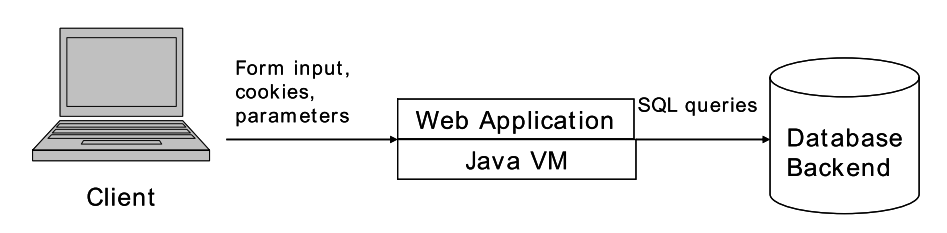
\includegraphics[width=\textwidth]{images/webApplication-Haldar.png}
  \caption{An illustration of the three-tier architecture commonly used by web applications \cite{Haldar}.}
  \label{fig:webApplication-Haldar}
\end{figure}

From Figure \ref{fig:webApplication-Haldar} it can be seen that tiers only communicate with the tiers closest to themselves. This causes the logic tier to become a safeguard for the storage tier where valuable and possibly sensitive information is stored. The sensitive information might, for example, be users name, email, personal security numbers and credit card information \parencite{JustinClarke-Salt2009SIAa}.

The scope of the thesis lies in the logic tier where both trusted and untrusted data is processed, and validations are needed to ensure secure applications. The programming language for the logic tier can vary a lot, but one common and the chosen language for this thesis is Java.



\subsection{Structured Query Language}
Communication between the logic and storage tier is done through a standardized language called Structured Query Language, mostly known as SQL. SQL is created to manipulate and access databases programmatically. The majority of today's database uses SQL. The language works by building queries specifying the required information or task. The query is then evaluated and handled up upon by the SQL engine \parencite{DarieCristian2003TPGt}.



\section{CIA Triad}
\label{cia}
Discussions regarding information security often rely on the CIA Triad. CIA stands for confidentiality, integrity, and availability as displayed in Figure \ref{fig:CIATriad}. Confidentiality ensures data usage by only authorized individuals. Integrity specifies that application data should be accurate and unaltered. Availability is the ability to access the application and application data \parencite{2014C1-W}.

\begin{figure}[H]
    \centering
    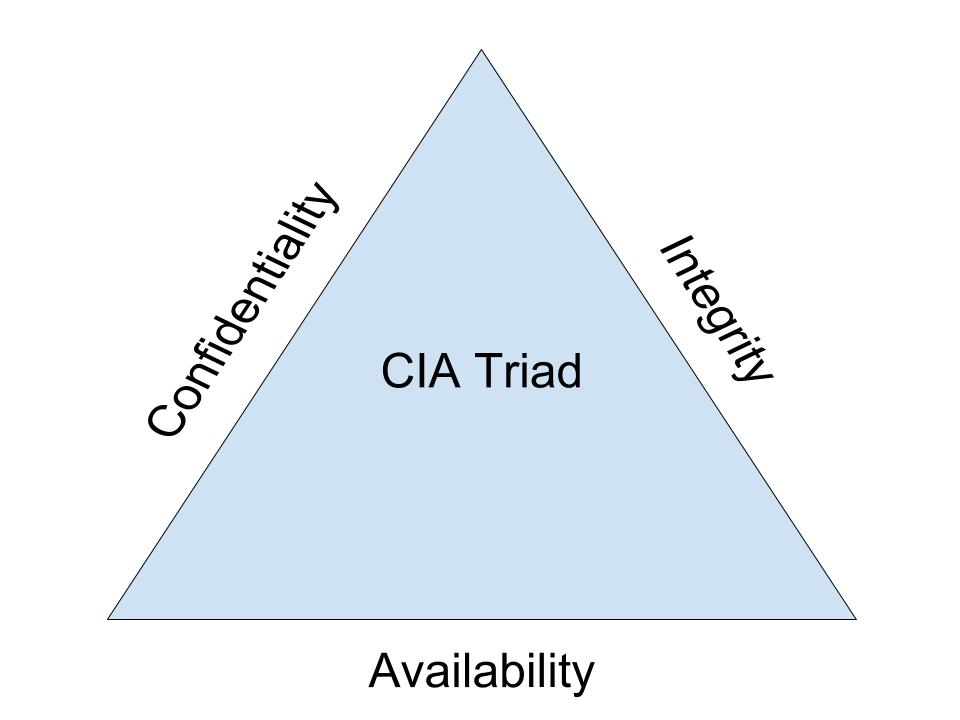
\includegraphics[height=6cm]{images/CIATriad.jpg}
    \caption{An illustration of the CIA Triad, model used when discussing information security.}
    \label{fig:CIATriad}
\end{figure}



\section{Security Vulnerabilities}
\label{SecurityVulnerabilities}
The organization Open Web Applications Security Project, known as OWASP, is an online community which aims to provide knowledge on how to secure web applications \parencite{OpenWebApplicationSecurityProject}. OWASP has produced reports about the top ten security risks for web applications, and the latest was published in 2017. The report contains information about the ten most common security risks for the given year. Information such as how the security risk is exploited and possible prevention methods are also presented. This thesis will look at security risk number one and seven from the latest report. These two security risks are vulnerabilities of information disclosure and code injection. The two vulnerabilities are Injection attack and Cross-Site Scripting \parencite{OWASP2017}.



\subsection{SQL Injection Attacks}
The most common security risk is Injection Attacks \parencite{OWASP2017}. Injection Attack is an attack where the attacker's input changes the intent of the execution. The typical results of Injection Attacks are file destruction, lack of accountability, denial of access and data loss \parencite{Secure_Web}.

Injection Attacks exists towards a broad set of different areas but the area discussed and analyzed in this thesis is SQL Injections. SQL Injections can be divided into two different subgroups. These two subgroups are SQL Injection and Blind SQL Injection \parencite{Secure_Web}.



\subsubsection{SQL Injection}
SQL Injection occurs when an SQL query is tampered with which results in gaining content or executing a command on the database which was not intended. Listing \ref{lst:acceptable_to_SQL_Injection} displays an SQL query which is open to SQL Injections. This is because the variable UserId is never validated before it is propagated into the query \parencite{JustinClarke-Salt2009SIAa, Secure_Web}.

\hfill
\begin{lstlisting}[
  language=SQL,
  caption=Pseudo code acceptable to SQL Injection through malicious usage of \textit{userInput}.,
  label={lst:acceptable_to_SQL_Injection}]
userId = (*@\textit{userInput}@*)
"SELECT * FROM Users WHERE userId = " + userId
\end{lstlisting}
\hfill

The query work as intended if the user input, labeled as \textit{userInput}, is a valid Integer (since Integer is what we have decided that user id is in the application). An example of malicious usage of user input is \textit{10 or 1 = 1}. This input would result in the query seen in Listing \ref{lst:SQL_Injection}.

\hfill
\begin{lstlisting}[
  language=SQL,
  caption=An example of SQL Injection where the whole Users table is returned,
  label={lst:SQL_Injection}]
SELECT * FROM Users WHERE userId = 10 or 1 = 1
\end{lstlisting}
\hfill

This query results in an execution that always evaluates to true. As a result the query returns the whole table of users. This problem can be prevented in different ways. The first is through validation of input. By verifying user input as in Listing \ref{lst:SQL_Injection_Verified} can we protect the query from being vulnerable to the SQL Injection.

\hfill
\begin{lstlisting}[
  language=SQL,
  caption=An example of SQL Injection prevention through variable sanitiazion.,
  label={lst:SQL_Injection_Verified}]
userId = (*@\textit{userInput}@*)
isInteger(userId)
"SELECT * FROM Users WHERE userId = " + userId
\end{lstlisting}
\hfill

A second common alternative is to use SQL Parameters which handle the verification for the user. This leaves the verification and validation of input up to the SQL engine. An example written with SQL Parameters can be seen in Listing \ref{lst:SQL_Injection_Parameters}.

\hfill
\begin{lstlisting}[
  language=SQL,
  caption=An example of SQL Injection prevention through SQL Parameters.,
  label={lst:SQL_Injection_Parameters}]
userId = (*@\textit{userInput}@*)
sqlQuery = "SELECT * FROM Users WHERE userId = @0"
db.Execute(sqlQuery, userId)
\end{lstlisting}



\subsubsection{Blind SQL Injection}
Blind SQL Injection is very similar to SQL Injection. The only difference is that the attacker does not receive the requested information in clear text from the database. The information is instead received by monitoring variables such as how long time the response takes or what kind of error messages it returns. An example of the first is an SQL query that tells the SQL engine to sleep depending on a condition. An example of this can be seen in Listing \ref{lst:Blind_SQL_Injection_Time} \parencite{JustinClarke-Salt2009SIAa, Secure_Web}.

\hfill
\begin{lstlisting}[
  language=SQL,
  caption=An example of Blind SQL Injection where query response is delayed five seconds if a user with id one is in the Users table.,
  label={lst:Blind_SQL_Injection_Time}]
SELECT * FROM Users WHERE userId = 1 WAITFOR DELAY '0:0:5'
\end{lstlisting}
\hfill

The second variant of a Blind SQL Injection is through analyzing error messages and, depending on what they return, build an image of the targeted data. This is mostly done through testing different combinations of true and false queries \parencite{JustinClarke-Salt2009SIAa, Secure_Web}.



\subsection{Cross-Site Scripting}
Cross-Site Scripting has been a vulnerability since the introduction of JavaScript in websites. One of the first Cross-Site Scripting attacks was carried out just after the release. The attack was conducted through loading a malicious web application into a frame on the site that the attacker wants to gain access to. The attacker could then through JavaScript access any content visible or typed into the web application. Same-Origin Policy was introduced to prevent this form of attacks. The policy restricts JavaScript to only access content from its origin \parencite{FogieSeth2007Xacs, w3csop}.

The introduction of the Same-Origin Policy, however, did not stop the attackers. The next wave of attacks was mostly towards chat rooms where it was possible to inject malicious Cross-Site Scripts into the message input form. Which would then be reflected by the server itself, when displaying the message for other users, and thereby bypassing the Same-Origin Policy \parencite{FogieSeth2007Xacs}.

There are three different types of Cross-Site Scripting. These three are reflected, stored, and DOM-based Cross-Site Scripting.



\subsubsection{Reflected Cross-Site Scripting}
Reflected Cross-Site Scripting, mostly conducted through a malicious link that an user accesses. The malicious link will exploit a vulnerable input on the targeted web application and through the input reflect back malicious content to the user \parencite{Secure_Web}.



\subsubsection{Stored Cross-Site Scripting}
Stored Cross-Site Scripting is when malicious scripts get stored in the targeted web applications database. This malicious script is then loaded and presented to each user who is trying to access the application \parencite{Secure_Web}.



\subsubsection{DOM-based Cross-Site Scripting}
DOM-based Cross-Site Scripting is very similar to Reflected Cross-Site Scripting, but it does not necessarily have to be reflected from the application server. DOM-based Cross-Site Scripting modifies the DOM tree and through that it exploits the user \parencite{Secure_Web}.



\section{Taint Tracking}
\label{DynamicTaintTracking}
Taint tracking, also known as taint analysis, is a tool to analyze the flow of information in an application \parencite{Pan2015}. The goal of taint tracking is to prevent possible attacks such as Injection and Cross-Site Scripting by enforcing the usage of sanitizers on input data. Taint tracking can be implemented in two different forms: static and dynamic. Static taint tracking is an evaluation tool possible to be included in the integrated development environment where it notifies the developer of possible security vulnerabilities. Dynamic taint tracking is a tool used simultaneously as the application execution. Dynamic tracking analyses for vulnerabilities at runtime and achieve higher accuracy compared to static tracking. The advantage for static is the ability to execute before runtime, but its disadvantage is the lower accuracy in tracking of taint.

Taint trackers operate by tracking untrusted data and acting upon any that are trying to enter sinks without first being sanitised. Perl and Ruby are two programming languages which have adapted to use taint checking \parencite{perl, ruby}. There are some tools which enable taint checking for other platforms. TaintDroid \parencite{Ma2010} for the Android platform is one of them. This thesis will discussion dynamic taint tracking and how it can improve the security of Java-based web applications.

Taint tracking contains four main steps which are described in Table \ref{table:taintTracking}. The first step is marking all data from untrusted sources as tainted. This is done through a taint flag attached to the input variables. Step two is tracking tait where tainted data propagates onto all data it comes in contact with. The third step is the possibility of detainting data, but this is only done after the data have been sanitized through predefined sanitizers. The fourth and last step is checking the taint flags in areas called sinks which are entry points to sensitive code \parencite{Pan2015, Venkataramani2008}. The decision of what to do if a tainted variable tries to pass through a sink varies depending on the application, however, remedial actions should be conducted. These actions should be, depending on the application owners choice, logging the events, throwing an error, or modifying the tainted values into safe predefined values. 

\begin{table}[H]
  \centering
  \caption{The four core tasks behind taint tracking.}
  \label{table:taintTracking}
  \begin{tabular}{rp{8.5cm}}
    \textbf{Tainting}           & Marking all data from sources as tainted.                          \\
    \textbf{Propagat Taint}     & Propagating taint to all data coming in contact with tainted data. \\
    \textbf{Detainting}         & Marking all data from sanitizers as non-tainted.                   \\
    \textbf{Assert Non-tainted} & Assert that data passing through sinks are non-tainted.           
  \end{tabular}
\end{table}

An example of taint tracking can be seen in Listing \ref{lst:taint_propagation}. In this example \textit{getAttribute} is a source, \textit{executeQuery} is a sink and \textit{validate} is a sanitizer. On line 1, the input from the source is flagged as tainted, and the taint propagates onto \textit{userId}. The sanitizer on line 2 validates \textit{userId} and removes the tainted flag. Lastly, the sink on line 3 executes the query since the argument is not tainted. If a user sends in a malicious userId containing "101 OR 1 = 1" the validator would sanitize the String and safely execute the sink command. However, removing line two would result in tainted data entering the sink. Without a dynamic taint tracker this would result in giving the malicious user the entire list of Users. With a dynamic taint tracker, however, the result is the sink halting the execution, therefore, preventing unwanted information disclosure.

\hfill
\begin{minipage}[H]{\linewidth}
\begin{lstlisting}[
  caption=A code example of accurately handling user input before accessing sensitive code area.,
  numbers=left,
  label={lst:taint_propagation}]
userId = getAttribute("userId");
validate(userId)
executeQuery("SELECT * FROM Users WHERE userId = " + userId);
\end{lstlisting}
\end{minipage}
\hfill



\section{Java}
\label{JavaInstrumentation}
Java has been around since the early 90's. The founder's objective was to develop a new improved programming language that simplified the task for the developers but still had a familiar C/C++ syntax. \parencite{OracleVoice}. Today is Java one of the most common programming languages \parencite{octoverse}.

Java is a statically typed language which means that no variable can be used before being declared. The variables can be of two different types: primitives and references to objects. Among the primitive types does Java have support for eight. These are byte, short, int, long, float, double, boolean and char \parencite{primjav}.



\subsection{Java Virtual Machine}
There exists a plethora of implementations of the Java Virtual Machine, but the official developed by Oracle is HotSpot \parencite{hotSpot}. One of the core ideas with Java during its development was "Write once, run anywhere." The slogan was created by Sun Microsystems which at the time were the company developing Java and the Java Virtual Machine. \parencite{Craig_2006}. The idea behind the Java Virtual Machine was to enable one language to be platform independent and then modify the Java Virtual Machine to run on as many platforms as possible. The Java Virtual Machine is a virtual machine with its own components of heap storage, stack, program counter, method area, and runtime constant pool.

Figure \ref{fig:JVM} illustrates the architecture of the Java Virtual Machine. The Class Loader loads the compiled Java code and adds it into the Java Virtual Machine Memory. The Execution Engine reads the loaded bytecode from the Java Virtual Machine Memory and executes the application instructions. The Java Virtual Machine have built in support for Java Agents which is a tool running between the Java Virtual Machine and the executed Java application. An Agent is loaded and given access to the application by the Class Loader. The Class Loader will trigger the implemented Java Agent and allow for instrumentation of each class file loaded by the Class Loader before being loaded into the Java Virtual Machine \parencite{venners_1999, instru}.

\begin{figure}[H]
  \centering
  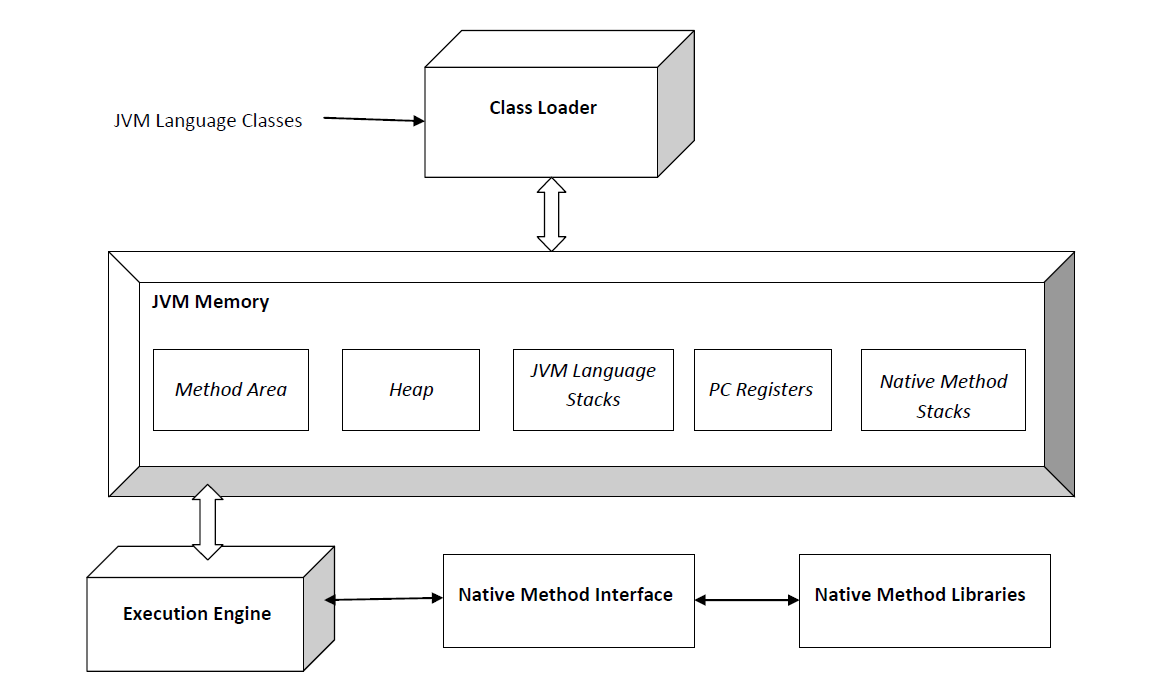
\includegraphics[width=\textwidth]{images/JvmSpec7.png}
  \caption{An illustration of the Java Virtual Machine Architecture \parencite{jvm}. }
  \label{fig:JVM}
\end{figure}


\subsection{Instrumentation}
Java instrumentation is a way to modify the execution of an application without knowing or modifying the application code itself. Good use cases for Java instrumentation are, for example, monitoring agents, event loggers, and taint trackers. Instrumentation is an official Java package that provides services needed to modify the bytecode of program instructions. It is conducted through implementing an Agent that makes it possible to transform every class loaded by the Class Loader before being used for the first time. However, there is a library of classes which cannot be instrumented by an Agent. This library is the rt.jar containing the Base Java Runtime Environment which is needed to start up the Java Virtual Machine including the Class Loader. Instrumentation of the Base Java Runtime Environment need to be done before running the Java application.

The Java Agent operates on bytecode which is time consuming work for the developer. To ease the task of instrumentation is the bytecode instrumentation library Javassist used \parencite{Java_Instrument, Javassist}.



\subsection{Javassist}
There exist several libraries that can help the developer in the task of creating a Java Agent. The help comes in libraries of methods to manipulate Java bytecode. The library used in this thesis is Javassist. Javassist stands for Java programming Assistant and provides two levels of API. The two are on source respectively bytecode level. We used the source level API which is providing functionality of manipulating Java bytecode with little bytecode knowledge \parencite{Javassist}.

The Javassist source level API provides classes representing instances of classes, methods and fields. These API classes contains methods to use when computing if the given class, method or field should be instrumented. The classes representing methods do also contain the methods \textit{insertBefore}, \textit{insertAfter​} or \textit{insertAt}. The three methods allows to insert Java code to the beginning, the end or at a specific position of the method.